\capitulo{3}{Conceptos teóricos}

\section{KNIME}

KNIME es un software de código abierto orientado a la ciencia de datos. A través de una interfaz gráfica intuitiva, 
permite crear flujos de trabajo de análisis de datos y minería de datos. KNIME fue desarrollado en la Universidad de 
Konstanz (Alemania) en 2004, y su nombre proviene de su denominación en inglés <<\english{Konstanz Information Miner}>>\cite{knime-whitepaper}. 
\

\begin{figure}[!h]
	\centering
	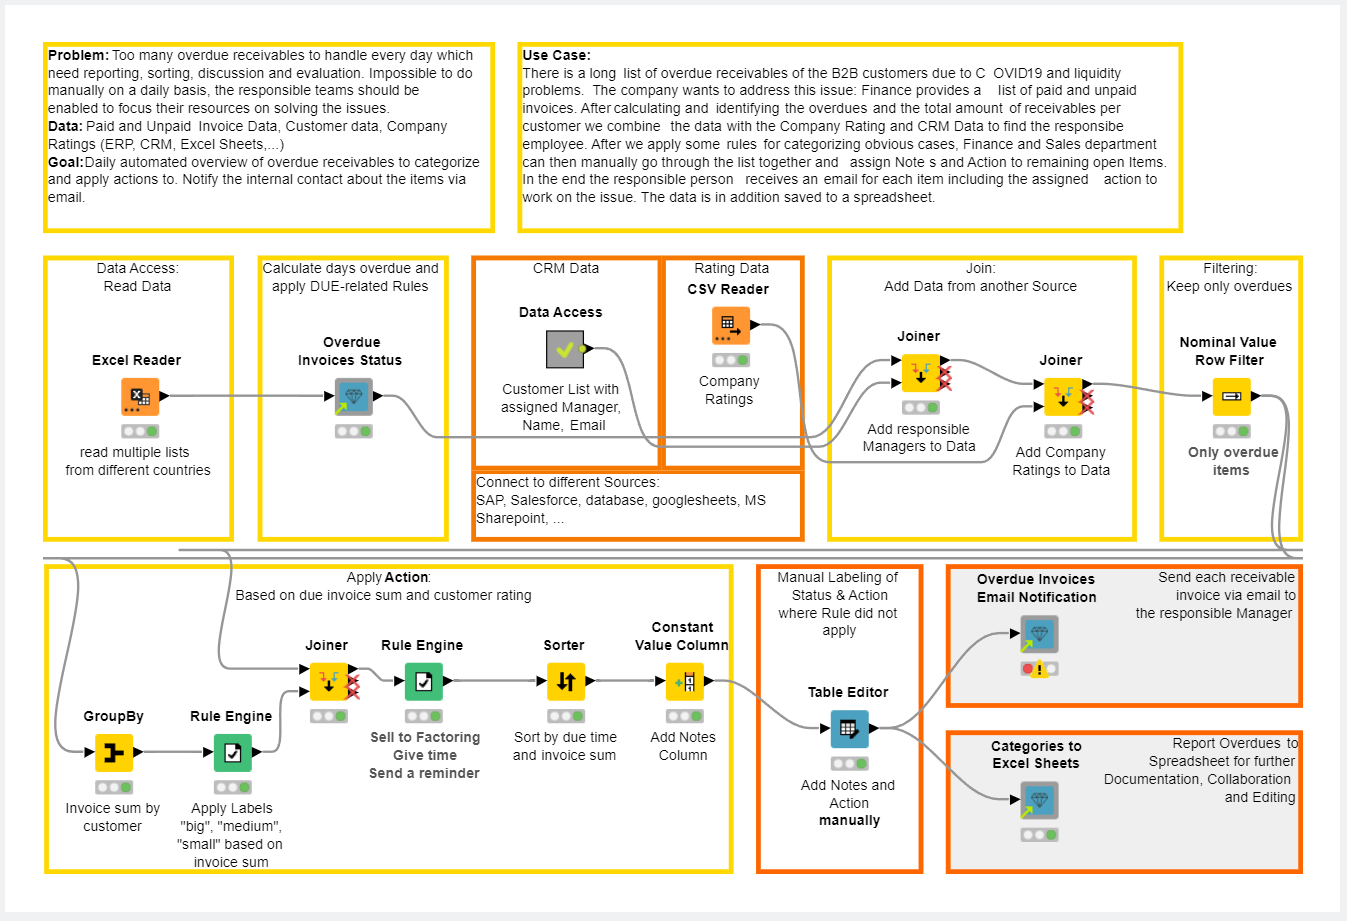
\includegraphics[width=1\textwidth]{img/3_ejemplo_workflow_knime.png}
	\caption{Ejemplo de Workflow en KNIME.}
	\label{fig:ejemploworkflow}
\end{figure}
\FloatBarrier

KNIME está concebido como una herramienta gráfica y dispone de una serie de nodos, que encapsulan distintos tipos de
 algoritmos, y flechas, que representan flujos de datos, que se despliegan y combinan de manera gráfica e interactiva.
\

KNIME cuenta con un \href{https://hub.knime.com/}{repositorio abierto} desde donde se pueden descargar nodos, \english{workflows}, componentes y extensiones. 
\

KNIME incluye más de 2000 nodos nativos, que puede extenderse con otros más de 4500 nodos disponibles en el \english{hub} 
de la comunidad. Cubre prácticamente todos los aspectos de la ciencia de datos, desde recopilar y manipular 
datos hasta darles sentido con técnicas sofisticadas de modelado y visualización.
\

El carácter abierto de la herramienta hace posible su extensión mediante la creación de nuevos nodos que 
implementen algoritmos a la medida del usuario. Además, existe la posibilidad de utilizar llamadas directas a Weka y 
o de incorporar de manera sencilla código desarrollado en R o Python.
\

Además de la versión \english{Community}, que es libre y gratuita, KNIME ofrece soluciones de pago para empresas, como \english{KNIME Server} 
y \english{KNIME Business Hub}. Estas soluciones se pueden instalar en los servidores del cliente y están diseñadas para la 
colaboración en equipo, la automatización, la gestión y el despliegue de flujos de trabajo. En este proyecto nos centraremos únicamente
en la versión \english{Community}. 
\

En la arquitectura de KNIME se compone principalmente de los siguientes elementos: 

\begin{itemize}
	\item \textbf{Nodos}. Un nodo representa una función específica que se aplica a los datos. Los nodos tienen conexiones de
	 entrada y salida para conectarse y comunicarse entre ellos. Los nodos realizan operaciones específicas, 
	 como lectura de datos, preprocesamiento, análisis, visualización o exportación de datos. 
	\item \textbf{Workflows}. Un \english{workflow} o flujo de trabajo es una representación visual de un conjunto de operaciones que se realiza 
	mediante nodos interconectados. 
	\item \textbf{Componentes}. Los componentes son nodos que contienen un subflujo de trabajo, lo que nos permite agrupar 
	funciones para reutilizar en diferentes flujos de trabajo. 	
	\item \textbf{Metanodos}. Los metanodos se utilizan para simplificar los flujos de trabajo. Se trata de seleccionar una parte del flujo, 
	compuesta por varios nodos y sus relaciones, y agruparlos en un nodo especial llamado metanodo, con lo que ocultamos esa parte del flujo 
	y lo simplificamos visualmente. En cualquier momento podemos volver a expandir el metanodo para visualizar esa parte del flujo. 
	\item \textbf{Extensiones}. Las extensiones son \english{plugins} adicionales que podemos añadir a KNIME para ampliar las funcionalidades que 
	no están incluidas en el núcleo. Generalmente las extensiones incluyen nodos agrupados dentro de una misma temática. 
\end{itemize}

\section{Moodle}

Moodle es una plataforma de gestión del aprendizaje (\english{LMS, Learning Management System}) de código abierto diseñada
 para crear y administrar cursos en línea. Moodle se ha convertido en una de los LMS más populares y ampliamente 
 utilizados en todo el mundo, con una importante presencia en el ámbito universitario.
\

Moodle registra en sus \english{logs} una gran variedad de información. Para este proyecto nos centraremos únicamente en 
la información que Moodle recopila relacionada con el proceso de enseñanza-aprendizaje, como puede ser: 

\begin{itemize}
  \item Registro de actividad del usuario. En estos \english{logs} se registra la actividad de los usuarios, como cuándo 
  acceden a la plataforma, cuándo ven o completan módulos de cursos, cuándo participan en foros de discusión y
   cuándo envían tareas o cuestionarios. 
  \item Registro de calificaciones en tareas y cuestionarios.
  \item Registro de mensajes y comunicación. Los \english{logs} pueden registrar la comunicación entre usuarios, 
  como mensajes internos, mensajes de foros de discusión y chat en vivo.
\end{itemize}



\section{ETL}

ETL (\english{extract, transform, load}) \cite{etl} es un proceso de tres fases en el que los datos se extraen, se transforman y se cargan en un 
contenedor de datos de salida. Los datos pueden obtenerse de una o varias fuentes y enviarse a uno o varios destinos.

\begin{itemize}
	\item \textbf{Extracción}. En esta primera fase se extraen los datos en bruto de diferentes fuentes. En este proyecto los datos 
    provienen principalmente de Moodle aunque son extraídos usando diferentes técnicas (servicios web y \english{web scraping}). 
	\item \textbf{Transformación}. En esta fase se aplican una serie de transformaciones para preparar y limpiar los datos antes de 
	ser cargados para su uso. En este proyecto se realizarán transformaciones como la anonimización de datos personales, 
    obtención del género del usuario, obtención de información de los \english{logs} de eventos, etc.     
	\item \textbf{Carga}. En esta última fase se cargan los datos en un almacén o destino final. En este proyecto ese destino final son 
	los nodos de KNIME, que almacenan la información ya transformada y facilitan los datos en forma de tabla a través de un puerto de salida. 
\end{itemize}



\section{Aprendizaje supervisado}

El aprendizaje supervisado es un tipo de enfoque en el campo del aprendizaje automático, que es una rama de la inteligencia artificial. 
En el aprendizaje supervisado, un algoritmo o modelo se entrena utilizando un conjunto de datos etiquetados. 
Estos datos etiquetados consisten en ejemplos de entrada junto con las salidas o etiquetas deseadas. 
El objetivo del aprendizaje supervisado es generar un modelo que permita 
predecir las etiquetas de nuevas entradas de datos no etiquetadas.
\

De forma simplificada, podemos decir que el proceso de aprendizaje supervisado consta de las siguientes etapas \cite{aprendizaje}: 

\begin{enumerate}
	\item \textbf{División de datos para entrenamiento y pruebas}. Se recopila un conjunto de datos que contiene ejemplos de entrada 
	junto con las etiquetas correctas. El conjunto de datos etiquetados se divide en dos subconjuntos principales: 
	el conjunto de entrenamiento (\english{training set}) y el conjunto de prueba (\english{test set}). 
    \item \textbf{Entrenamiento del modelo}. Se utiliza el conjunto de datos de entrenamiento (generalmente sobre
	 el 70-80\% de los datos) para entrenar el modelo de aprendizaje automático, en busca de patrones y relaciones en los datos
	  que le permitan hacer predicciones precisas.
	\item \textbf{Prueba y evaluación}. Una vez que el modelo está entrenado, se prueba con la parte de los datos etiquetados 
	que no se usaron en el entrenamiento del modelo (conjunto de \english{test} o prueba). Esto permite evaluar la capacidad del 
	modelo para hacer predicciones. En esta etapa se calcula la precisión del modelo, obtenida mediante la comparación de
	 las predicciones del modelo con las etiquetas reales en los datos de prueba.
	\item \textbf{Uso en la predicción}. Después de que el modelo ha sido entrenado y evaluado satisfactoriamente, 
	puede utilizarse para hacer predicciones sobre nuevas entradas desconocidas o no etiquetadas. 
\end{enumerate}

